\documentclass{article}

\textwidth=6.5in
\textheight=8.5in
\voffset=-54pt
\oddsidemargin=0in
\evensidemargin=0in
\setlength{\parskip}{8pt}
\setlength{\parindent}{0pt}

\usepackage{amsmath, amssymb}
\usepackage{ifthen}

\usepackage[inline]{enumitem}
\setlist{topsep=0pt, parsep=8pt}

\usepackage[rgb,table]{xcolor}\convertcolorsUfalse
\usepackage{graphicx}

% change hyperref options
\PassOptionsToPackage{hyphens}{url}
\usepackage[bookmarks,colorlinks,linkcolor=black,citecolor=blue,pdfstartview=FitH,urlcolor=blue]{hyperref}
\hypersetup{pdfpagemode=UseNone}
\usepackage{bookmark}

\usepackage{graphicx}
\usepackage{multicol}
\usepackage{framed}
\usepackage{array}

\usepackage{icomma}

\usepackage{soul}
\usepackage[normalem]{ulem}

\usepackage{pgfplots}
\pgfplotsset{compat=1.18}  
\pgfplotscreateplotcyclelist{mycolor}{black, blue, red, green!70!black, magenta, purple, cyan, orange }  
\pgfplotsset{
  disabledatascaling,
  cycle list=tikzcolor, 
  axis lines=middle,
  every axis plot/.style={no marks, thick},
  every axis/.style={
    enlarge x limits=false,
    enlarge y limits=auto,
    xlabel style={at={(current axis.right of origin)},anchor=west},
    ylabel style={at={(current axis.above origin)},anchor=south},
    % extra x and y ticks for asymptotes
    extra x tick style={grid=major, grid style={dashed,black}},
    extra y tick style={grid=major, grid style={dashed,black}},
    /pgf/number format/1000 sep={},
  },    
  tick label style = {font=\footnotesize, fill=\currentbgcolor, inner sep=0pt},    
  xticklabel shift=1pt,    
  scaled ticks=false,
  scaled y ticks=false,
  unbounded coords=jump,
  samples=101,
  minor tick length=0,
  scatter/classes={
    open={mark=*,draw=black,fill=white, mark size=2, thin},
    closed={mark=*,draw=black,fill=black, mark size=2, thin}
  },
  width=3in,
}
\pgfplotsset{open/.style={only marks, mark=*, fill=white, thin, mark size=2}}
\pgfplotsset{closed/.style={only marks, mark=*, draw=black, fill=black,
    thin, mark size=2}}
\pgfplotsset{labeled/.style={nodes near coords, only marks, mark=*, draw=black, fill=black, thin, mark size=2, point meta=explicit symbolic}}

\pgfplotsset{gridgraph/.style={clip=false, axis line style={shorten
      >=-8pt}, xlabel style={xshift=8pt}, ylabel style={yshift=8pt},
    enlargelimits=false, grid=major, tick style={black}}} 

\usepackage{tikz}
\usetikzlibrary{
  matrix,%
  % enables the snake paths
  decorations.pathmorphing,%
  % enables bigger arrows
  decorations.markings,%
  decorations.pathreplacing,%
  decorations.text,%
  calc,%
  patterns,%
  shapes.geometric,%
  arrows,
  decorations.shapes,
  positioning,
  plotmarks,
  intersections
}
\tikzset{>=latex} % sets default arrow type in tikz
\tikzset{font=\normalsize}
\tikzset{mark size=1.5pt, mark options=thin}
\tikzset{pin distance=4pt,
  every pin edge/.style={<-, thin, shorten <= -2pt}}

\interfootnotelinepenalty=10000
\renewcommand{\thefootnote}{(\arabic{footnote})}

\usepackage{multirow, bigdelim}

% change to \usepackage[sols]{handout} to see solutions
\usepackage[]{handout}

\newcommand\iscurrentenumi[1]{%
  \ifthenelse{\equal{#1}{\theenumi}}{}{#1}}
\setenumerate[1]{ref=\#\arabic*}
\setenumerate[2]{ref=\protect\iscurrentenumi{\theenumi}(\alph*)}
\newcommand\enumiiprefix[2]{%
  \ifthenelse{{\equal{#1}{\theenumi}}\AND{\equal{#2}{(\alph{enumii})}}}{}{}%
  \ifthenelse{{\equal{#1}{\theenumi}}\AND{\NOT{\equal{#2}{(\alph{enumii})}}}}{#2}{}%
  \ifthenelse{\equal{#1}{\theenumi}}{}{#1#2}%
}
\setenumerate[3]{ref=\protect\enumiiprefix{\theenumi}{(\alph{enumii})}\roman*}

\newlength{\tipmargin}
\makeatletter

% underline links               
\let\@href=\href
\renewcommand{\href}[2]{\@href{#1}{\ul{#2}}}

\renewenvironment{framed}{
  \setlength{\tipmargin}{\textwidth-\linewidth}
  \advance\@totalleftmargin-\tipmargin
  \def\FrameCommand{\hspace{\tipmargin}\fbox}%
  \advance\linewidth\tipmargin
  \MakeFramed {\advance\hsize-\width \FrameRestore}%
}
{\endMakeFramed}

\let\@uhref=\href
\usepackage[style=verbose-ibid]{biblatex}
\let\@autocite=\autocite
\renewcommand{\autocite}[1]{
  \let\href=\@href
  \@autocite{#1}
  \let\href=\@uhref
}
\let\@autocites=\autocites
\renewcommand{\autocites}[2]{
  \let\href=\@href
  \@autocites{#1}{#2}
  \let\href=\@uhref
}
\bibliography{references}
\makeatother

\definecolor{purple}{rgb}{0.5,0,1.0}

\usepackage{fancyhdr}
\lhead{\textcolor{white}{This content is protected and may not be shared, uploaded, or distributed.}}
\rhead{}
\rfoot{\vspace*{\fill}\footnotesize\textcopyright{} \emph{Harvard Math Ma}}
\renewcommand{\headrulewidth}{0pt}
\pagestyle{fancy}
\begin{document}

\htitle{33. Linear Functions, Exponentials, and Logarithms in the Real World}

\begin{problemonly}
  \begin{framed}

You should be able to:
    \begin{itemize}[topsep=0pt,partopsep=0pt,parsep=8pt,itemsep=0pt]
    \item Assess how appropriate it is to use a linear or exponential model to model data.

    \item Interpret plots where an axis has a logarithmic scale. 

    \end{itemize}
  \end{framed}
\end{problemonly}

\begin{enumerate}
\item 

  \note{This isn't relevant to anything we're doing today; it's just to reinforce that this is a graph they should know.}

  \begin{problem}[1.5in]
    \emph{Warm up.} Sketch the graph of $f(x) = \ln x$.
  \end{problem}

  \begin{solution}
    \begin{center}
      \begin{tikzpicture}
        \begin{axis}[xmin=-10, xtick={1}, ytick=\empty]
          \addplot[domain=0:10] {ln(x)};
        \end{axis}
      \end{tikzpicture}
    \end{center}
  \end{solution}

\item  

  \note{This problem is meant to have students think about what makes a function linear or exponential, as well as to make the point that a function need not be either. (Here, neither seems like a good model.)}  

  \href{https://people.math.harvard.edu/~jjchen/mathma/docs/articles/hoka-shoes-running-deckers-ugly-sneakers.html}{This article} about the shoe brand Hoka says,
  \begin{quote}
    It took five years for Hoka’s sales to accelerate from less than \$3 million to more than \$100 million. It took six more to zoom past \$1 billion.
  \end{quote}

  \begin{enumerate}
  \item

    \note{Based on the given information, we can see that their sales aren't growing at a constant rate.}

    \begin{problem}[\vfill]
      Does it seem reasonable to model Hoka's sales as a linear function of time? Explain why or why not. 
    \end{problem}

    \begin{solution}
      No, because the rate of change of Hoka's sales isn't constant.
      The average rate of change in the first 5 years around
      19.4 million
      dollars per year, whereas the average rate of the change in the
      following 6 years was around 150 million dollars per year.
    \end{solution}

  \item

    \note{But they also aren't growing by a constant factor every 5 years.}

    \begin{problem}[\vfill\newpage]
      Does it seem reasonable to model Hoka's sales as an exponential function of time? Explain why or why not. 
    \end{problem}

    \begin{solution}
      No, because Hoka's sales aren't being multiplied by a constant
      factor every 5 years either. Over the first 5 years, the growth
      factor was around 33, whereas in the following six years,
      the growth factor was 10. 
    \end{solution}

  \end{enumerate}

\item  

  The following figure is reproduced from a study\autocite{Pharmacokinetics} of how cats metabolize a particular chemotherapy drug, cyclophosphamide. In the study, 6 cats were given the drug by IV, and the concentration of the drug in their plasma was measured frequently afterwards. 

  \begin{center} % \begin{axis}
    \begin{tikzpicture}
      \begin{semilogyaxis}[xlabel={time in hours after receiving drug by IV}, ylabel={average concentration of drug in 6 cats (ng/mL)}, xlabel style={text width=1.6in, align=center}, ylabel style={text width=1.75in, align=center}, xmin=0, ymin=0.1, ymax=10000, gridgraph, axis y line=left]
        % Note: these aren't the actual data points; they're reconstructed from an image in the paper
        \addplot+[closed] coordinates { (0.25, 7961.41199885089) (0.5, 5655.555225142415) (1, 2853.9446400919032) (2, 1146.5841675756224) (4, 207.41095118420955) (6, 33.47745810705735) (8, 5.720391367263847) };
      \end{semilogyaxis}
    \end{tikzpicture}
  \end{center}

  \begin{enumerate}
  \item

    \begin{problem}[\stretch{0.5}]
      What's strange about the vertical axis?  
    \end{problem}

    \begin{solution}
      The scale on the vertical axis is not linear, meaning
      that identical distances between the tick marks on the vertical axis
      do not correspond to the same amount of the dependent variable. 
      Instead, every time we move up a tick mark on the vertical axis, 
      the value of the dependent variable is multiplied by 10.
    \end{solution}

  \end{enumerate}
  Let $C(t)$ be the average concentration of the drug in ng/mL (nanograms per milliliter) in the 6 cats $t$ hours after being given the drug.

  \begin{enumerate}[resume]
  \item
    \note{Here, we can see that $C(0) \approx 10^4$, $C(2) \approx 10^3$ and $C(4)$ is between $10^2$ and $10^3$. That's enough to show us that $C(t)$ definitely isn't linear.}

    \begin{problem}[\stretch{0.15}]
      Based on the graph, what are approximate values of $C(0)$, $C(2)$, and $C(4)$? 
    \end{problem}

    \begin{solution}
      We can see that $C(0) \approx 10^4$, $C(2) \approx 10^3$ and $C(4)$ 
      is between $10^2$ and $10^3$.
    \end{solution}

    \begin{problem}[\nstretch{0.85}]
      The data points roughly lie on a straight line; is $C(t)$ roughly a linear function?
    \end{problem}

    \begin{solution}
      $C(t)$ definitely isn't a linear function. This is because
      the average rate of change from $t=0$ to $t=2$ is not the same
      as the average rate of change from $t=2$ to $t=4$.
    \end{solution}

  \item \label{log-linear-interpretation}

    \begin{problem}
      The true interpretation of the vertical axis is that it's showing a logarithm of the concentration. In this case, since the vertical axis has powers of 10, we're really seeing a graph of $\log_{10} C$. Label the values on the vertical axis.
    \end{problem}

    \begin{problemonly}
      \begin{center}
        \begin{tikzpicture}
          \begin{semilogyaxis}[xlabel={time in hours after receiving drug by IV}, ylabel={$\log_{10} C$}, xmin=0, ymin=0.1, ymax=10000, gridgraph, yticklabels={}, xlabel=$t$]
            % Note: these aren't the actual data points; they're reconstructed from an image in the paper
            \addplot+[closed] coordinates { (0.25, 7961.41199885089) (0.5, 5655.555225142415) (1, 2853.9446400919032) (2, 1146.5841675756224) (4, 207.41095118420955) (6, 33.47745810705735) (8, 5.720391367263847) };
          \end{semilogyaxis}
        \end{tikzpicture}
      \end{center}
    \end{problemonly}

    \begin{solution}
      \begin{center}
        \begin{tikzpicture}
          \begin{semilogyaxis}[xlabel={time in hours after receiving drug by IV}, ylabel={$\log_{10} C$}, xmin=0, ymin=0.1, ymax=10000, gridgraph, yticklabels={, $-1$, 0, 1, 2, 3, 4}, xlabel=$t$, axis y line=left]
            % Note: these aren't the actual data points; they're reconstructed from an image in the paper
            \addplot+[closed] coordinates { (0.25, 7961.41199885089) (0.5, 5655.555225142415) (1, 2853.9446400919032) (2, 1146.5841675756224) (4, 207.41095118420955) (6, 33.47745810705735) (8, 5.720391367263847) };
          \end{semilogyaxis}
        \end{tikzpicture}
      \end{center}
    \end{solution}

  \item

    \note{Here's the best-fit line for $\log_{10} C$: \url{https://www.desmos.com/calculator/b6shqcqqfg} We'll just eyeball something like $\log{10} C(t) \approx -0.4 t + 3.9$, and then I want them to solve for $C(t)$.}

    \begin{problem}[\stretch{0.15}]
      Based on the graph, write an approximate formula for $\log_{10} C(t)$. 
    \end{problem}

    \begin{solution}
      We can see that $\log_{10} C$ is roughly a linear function of $t$,
      $\log_{10} C \approx -0.4t+3.9$.
    \end{solution}

    \begin{problem}[\vfill]
      Use your formula for $\log_{10} C(t)$ to get an approximate formula for $C(t)$, and sketch a ``normal'' graph of $C(t)$. 
    \end{problem}

    \begin{solution}
      We can solve $\log_{10} C \approx -0.4t + 3.9$ for $C$:
      \begin{align*}
        \log_{10} C &\approx -0.4t + 3.9 \\
        C &\approx 10^{-0.4t + 3.9} \\
        C &\approx 10^{3.9} (10^{-0.4})^t \\
        C &\approx 8000(0.4)^t
      \end{align*}
      Therefore $C(t) \approx 8000(0.4)^t$. A ``normal'' graph would
      look like this.
      \begin{center}
        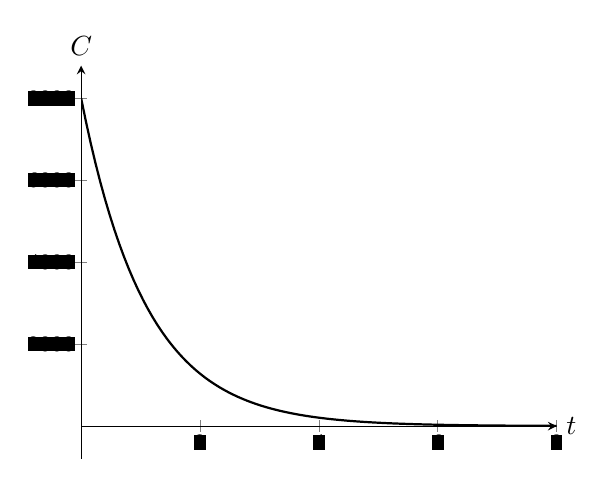
\begin{tikzpicture}
          \begin{axis}[ylabel=$C$, xlabel=$t$ ]
            \addplot[domain=0:8] {8000*0.4^x};
          \end{axis}
        \end{tikzpicture}
      \end{center}
      
    \end{solution}

  \item
    \begin{problem}[\nstretch{0.4}]
      This type of graph is called a \uline{log-linear} graph because the vertical axis is drawn using a logarithmic scale while the horizontal axis is drawn using a normal (``linear'') scale. If the log-linear graph of a function $f(x)$ is linear, what does that tell you about $f(x)$?
    \end{problem}

    \begin{solution}
      If a $\log_{b} y$ is a linear function of $x$, then $y$ is
      an exponential function of $x$.
      \begin{align*}
          \log_{b} y &= mx+c \\
          y &= b^{mx+c} \\
          y &= b^c (b^m)^x
      \end{align*}
    \end{solution}

  \end{enumerate}

\item  \label{semi-log-gd-153} Gadolinium-153 is a radioactive isotope used in X-ray fluorescence and osteoporosis screening. Suppose you have a sample of Gadolinium-153. Because it is radioactive, the amount of Gadolinium-153 in the sample naturally decays exponentially over time. Here is a log-linear plot of $G(t)$, the number of milligrams of Gadolinium-153 in the sample after $t$ days.

  \parbox[t]{2.4in}{\vspace{-8pt}
    \begin{tikzpicture}
      \begin{semilogyaxis}[gridgraph, ytick={1/4, 1/2, 1, 2, 4, 8}, xtick={240, 480, 720, 960}, yticklabels={$\frac{1}{4}$, $\frac{1}{2}$, 1, 2, 4, 8}, axis y line=left, xlabel=$t$, ylabel=$G$, width=2.6in]
        \addplot+[domain=0:960] {8 * (1/2)^(x/240)}; 
      \end{semilogyaxis}
    \end{tikzpicture}
  }  
  \begin{minipage}[t]{\linewidth-2.7in}
    \vspace{-8pt}
    \begin{enumerate}
    \item
      \begin{problem}[0.25in]
        What's the half-life of Gadolinium-153?  
      \end{problem}

      \begin{solution}
        From the plot, we can see that it takes 240 years for $G$
        to reduce by half, so the half-life is 240 years.
      \end{solution}

    \item

      \note{Here, we can use the half-life, or we can write a formula for $\log_2 G(t)$ and solve it to get $G(t)$.}

      \begin{problem}
        Write a formula for $G(t)$.
      \end{problem}

      \begin{solution}
        $G(t) = 8(2)^{-t/240}$.
      \end{solution}
    \end{enumerate}    
  \end{minipage}

  \pspace{0.25in}

  \begin{enumerate}[start=3]
  \item
    \begin{problem}[\vfill]
      At what time is the amount of Gadolinium-153 in the sample equal to 3 milligrams?
    \end{problem}

    \begin{solution}
      It's difficult to tell where $3$ is on the $y$-axis. Since
      the plot is log-linear, it's
      \textbf{not} halfway between $2$ and $4$. 
      So we need to solve the equation $8(2)^{-t/240} = 3$.
      \begin{align*}
        8(2)^{-t/240} &= 3 \\
        2^{-t/240} &= \tfrac{3}{8} \\
        -\tfrac{1}{240}t &= \log_2 \tfrac{3}{8} \\
        -\tfrac{1}{240}t &= \log_2 3 - \log_2 8 \\
        t &= -240(\log_2 3 - 3) \\
        t &= 720 - 240 \log_2 3
      \end{align*}
      So the amount of Gadolinium-153 in the sample is equal to $3$
      milligrams at $t=720-240\log_2 3$, or after approximately $340$ 
      years.
    \end{solution}

  \end{enumerate}

\item  
  % https://www.mdpi.com/2079-8954/2/2/89

  \note{Students will look more at this model in their homework (\#2). Here, I just want to talk about why people present data using logarithmic scales: if you use a regular plot, then most of the data gets crammed into the lower left corner. Here's an illustration showing just the elephant and man data points on a normal plot: \url{https://www.desmos.com/calculator/vn3kwvk8ju}}

  \begin{problem}[\newpage]
    Here's a figure from a paper\autocite{systems2020089} about how body size relates to metabolism in different animals. (This graph is known as the ``mouse-to-elephant curve''.) What do you notice about the axes? Why do you think the authors of this figure have chosen to present it this way rather than using a ``normal'' graph?

    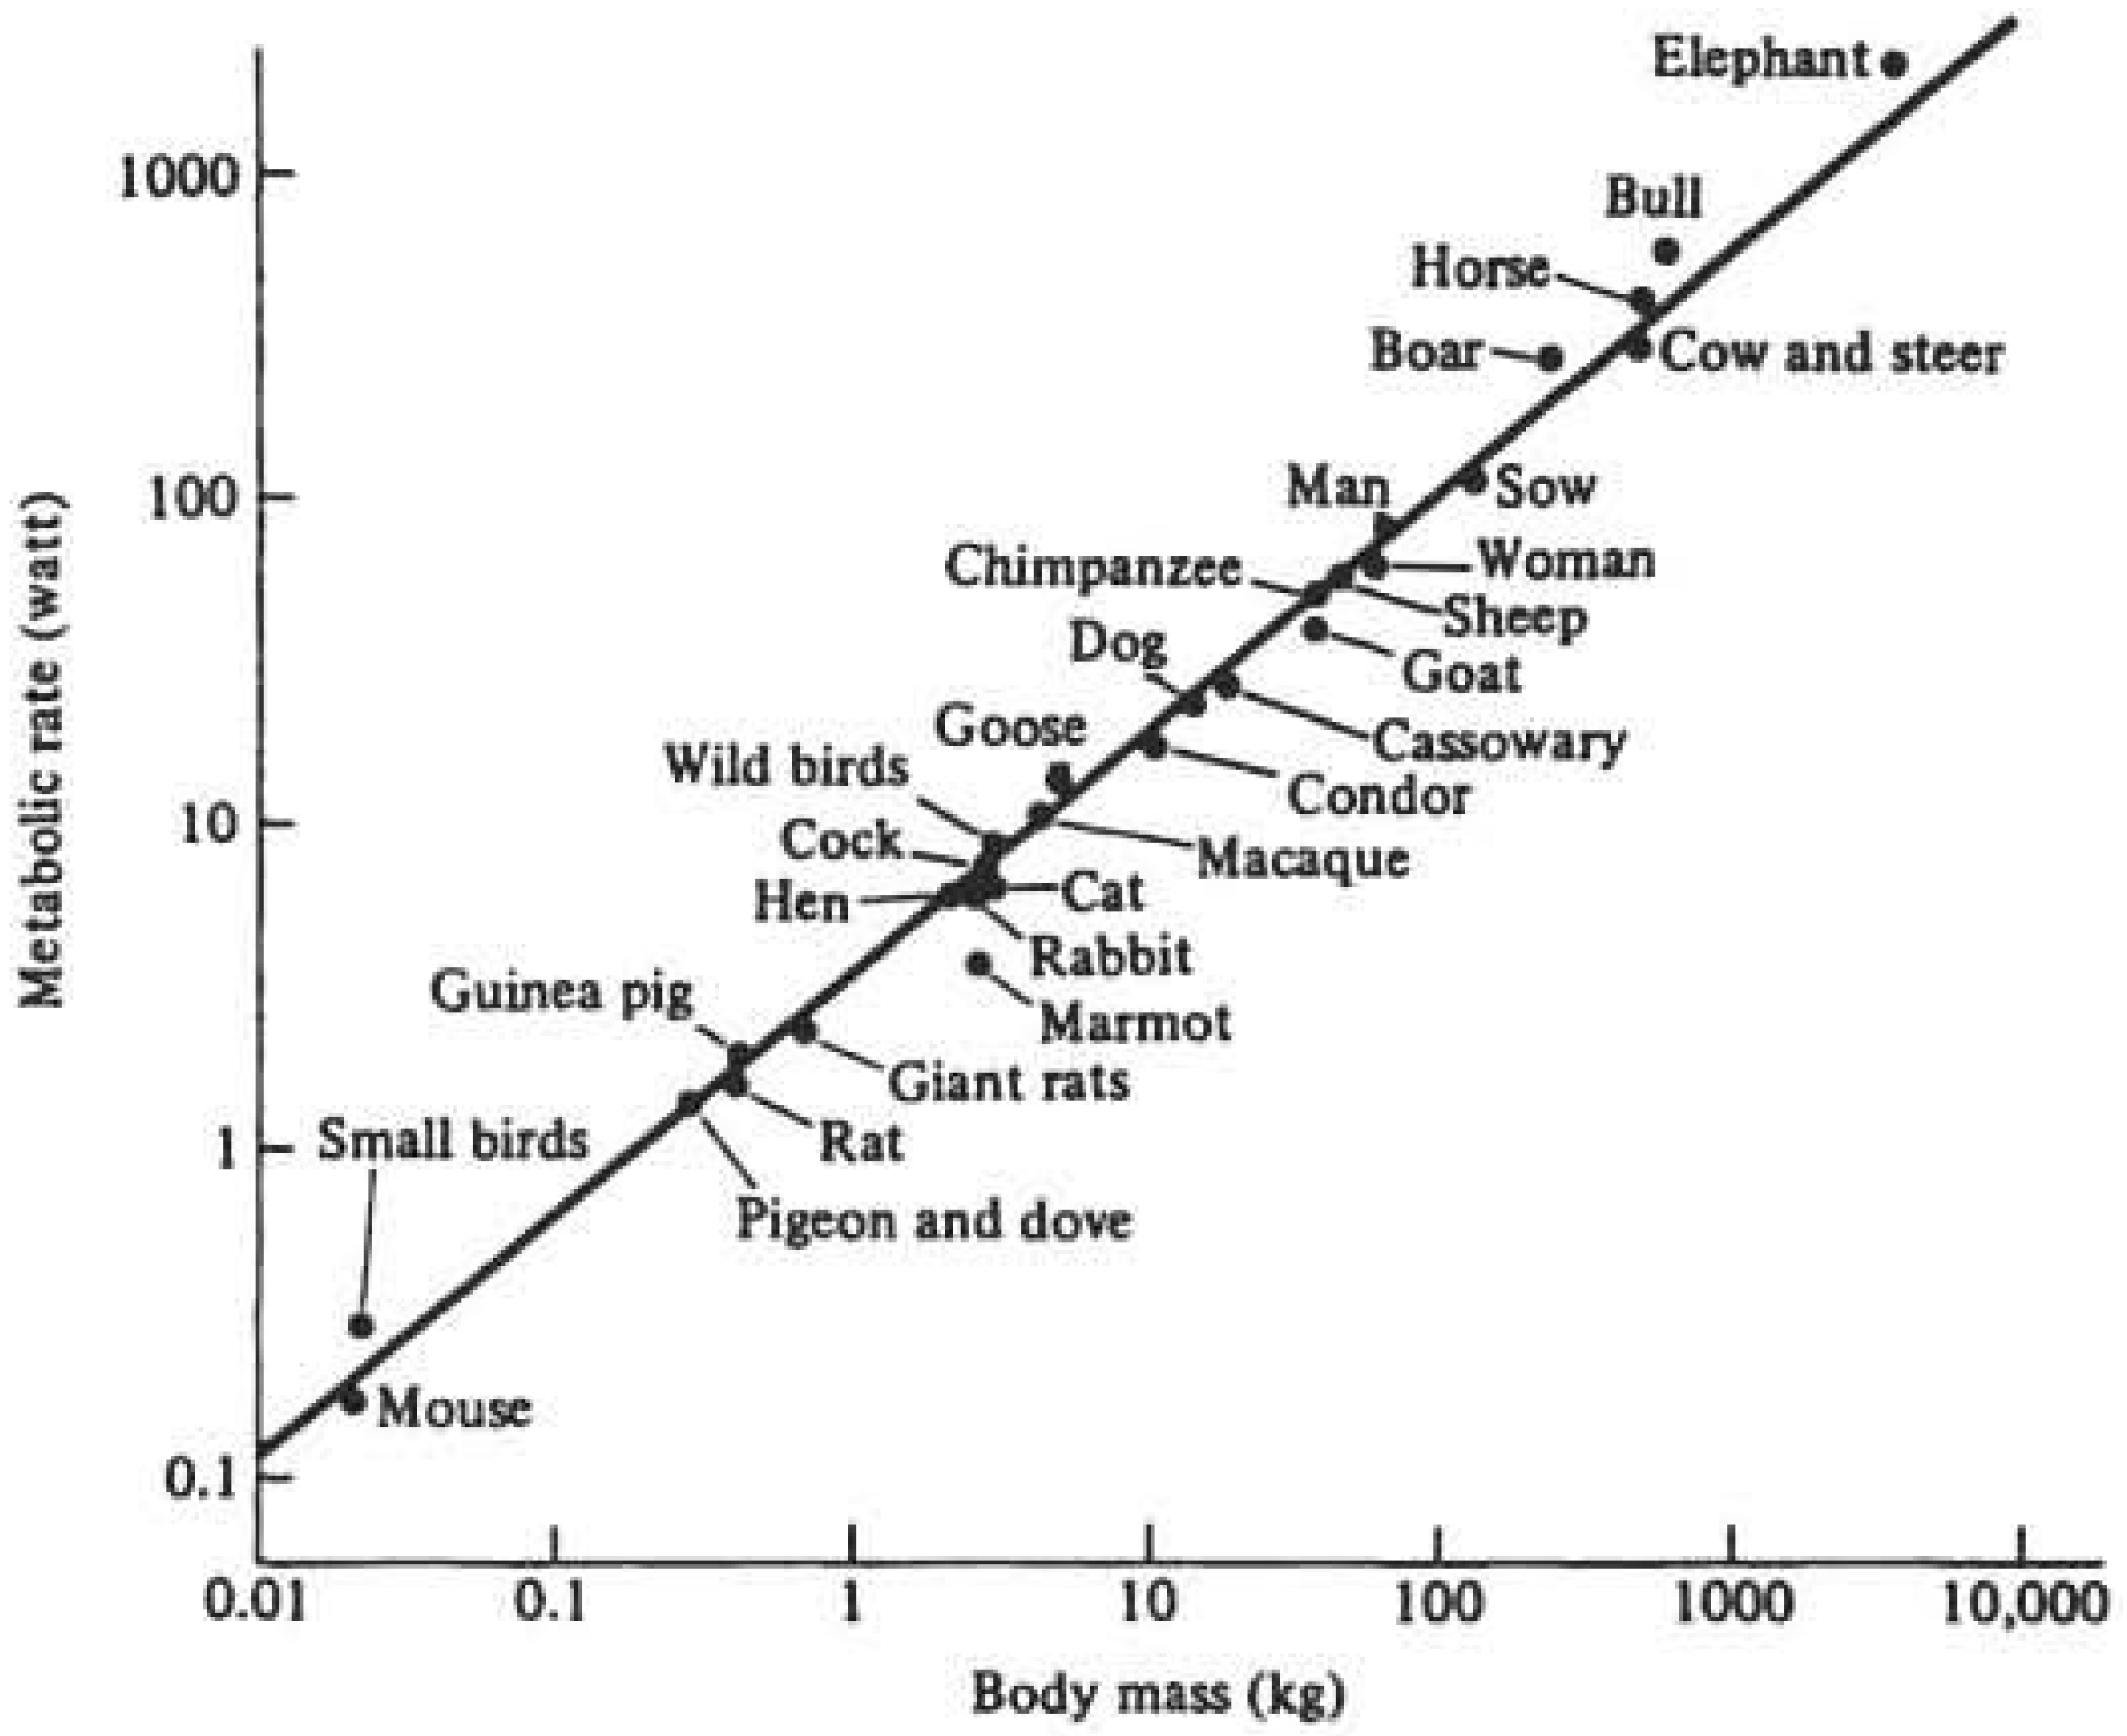
\includegraphics[scale=0.8]{images/systems-02-00089-g001.png}
  \end{problem}

  \begin{solution}
    We can see that both axes follow log scales. This is called a
    \textit{log-log plot}. The authors may have chosen to
    present the data this way in order to equally space out
    animals whose sizes are on different orders of magnitude, instead
    of having small animals be crammed into the lower-left corner. Also,
    the authors may have wanted to highlight the linear relationship
    between the logarithm of metabolic rate and the logarithm of
    body mass.
  \end{solution}

\item 

  \note{I hope we'll have time to start this, but it's okay if we don't; it doesn't have anything new.}

  Arturo is keeping an eye on a YouTube video; at noon, he sees that it has 1200 views. 10 minutes later, it has 1400 views. Arturo decides to write two models for the number of views $t$ minutes after noon, a linear model $L(t)$ and an exponential model $E(t)$. 

  \begin{enumerate}
  \item
    \begin{problem}[\vfill]
      Sketch graphs of $L(t)$ and $E(t)$ on the same axes. For what times does the linear model predict a higher number of views?
    \end{problem}

    \begin{solution}
      \begin{center}
        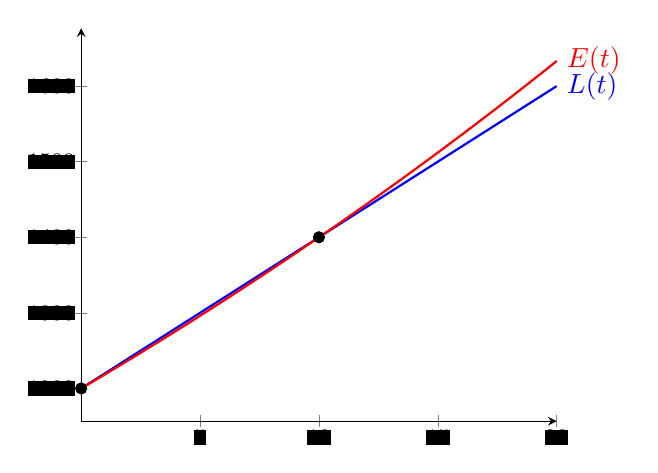
\begin{tikzpicture}
          \begin{axis}[clip=false]
            \addplot[closed] coordinates {(0,1200) (10, 1400)};
            \addplot[domain=0:20, blue] {1200+20*x} node[right] {$L(t)$};
            \addplot[domain=0:20, red] {1200*(7/6)^(x/10)} node[right] {$E(t)$};
          \end{axis}
        \end{tikzpicture}
      \end{center}
      The linear model predicts a higher number of views
      than the exponential model between $t=0$
      and $t=10$, and a lower number of views after $t=10$.
    \end{solution}

  \item
    \begin{problem}[\stretch{0.3}]
      Arturo wants to predict how quickly the number of views is increasing at 12:20 pm. Will the linear model or exponential model give a higher prediction? 
    \end{problem}

    \begin{solution}
      The exponential model will give a higher prediction
      for the rate at which the number of views is increasing
      at $t=20$.
    \end{solution}

  \item

    \note{Just a reminder that we really don't have any information that suggests whether either model is appropriate.}

    \begin{problem}[\stretch{0.3}]
      Do we have enough information to decide whether a linear or exponential function is an appropriate model? 
    \end{problem}

    \begin{solution}
      No. We only know enough to plot two points on the graph.
    \end{solution}

  \item
    \begin{problem}[\stretch{0.3}]
      According to the linear model, how quickly is the number of views changing at 12:20 pm?
    \end{problem}

    \begin{solution}
      The linear model is $L(t) = 1200 + 20t$, so $L'(20)=20$.
    \end{solution}

  \item
    \begin{problem}[\vfill\newpage]
      According to the exponential model, how long does it take for the number of views to reach $n$? And how would you express this quantity in function notation?
    \end{problem}

    \begin{solution}
      The exponential model is $E(t) = 1200(\tfrac{7}{6})^{t/10}$. We
      set this equal to $n$ and solve for $t$:
      \begin{align*}
        1200(\tfrac{7}{6})^{t/10} &= n \\
        (\tfrac{7}{6})^{t/10} &= \tfrac{n}{1200} \\
        \tfrac{1}{10}t &= \log_{7/6} \tfrac{n}{1200} \\
        t &= 10 \log_{7/6} \tfrac{n}{1200}
      \end{align*}
      This is the input of $E(t)$ when the output is $n$. In
      function notation, $E^{-1}(n)$.
    \end{solution}

  \item
    \begin{problem}[\vfill]
      According to the exponential model, how quickly is the number of views changing at 12:20 pm?
    \end{problem}

    \begin{solution}
      We want to find $E'(20)$, so we should first find $E'(t)$. We can 
      start by rewriting $E(t)$ as 
      $E(t) = 1200\left[(\tfrac{7}{6})^{1/10}\right]^t$, so
      \begin{align*}
        E'(t) &= 1200 \ln\!\left((\tfrac{7}{6})^{1/10}\right) 
        \left[(\tfrac{7}{6})^{1/10}\right]^t \\
        & =120\ln(\tfrac{7}{6})(\tfrac{7}{6})^{t/10}
      \end{align*}
      This means that
      $E'(20) = 120\ln(\tfrac{7}{6})(\tfrac{7}{6})^2$.
    \end{solution}

  \end{enumerate}

\item  Solve the following equations.

  \begin{enumerate}
  \item

    \begin{problem}[\vfill]
      $\ln(13 - 3x) - 2 \ln(3 - x) = 0$
    \end{problem}

    \begin{solution}
      \begin{align*}
        \ln(13 - 3x) - 2 \ln(3 - x) &= 0 \\
        \ln(13 - 3x) &= 2\ln(3-x) \\
        \ln(13-3x) &= \ln\!\left[(3-x)^2\right] \\
        13-3x &= (3-x)^2 \\
        13 - 3x &= x^2 - 6x + 9 \\
        0 &= x^2 - 3x - 4 \\
        0 &= (x-4)(x+1)
      \end{align*}
      This gives the two possible solutions $x=4$ and $x=-1$. However,
      $x=4$ is an extraneous solution since $\ln(3-x)$ is undefined
      when $x=4$. Thus, $x=-1$ is the only solution.
    \end{solution}

  \item
    \begin{problem}[\vfill]
      $2^{3x + 2} - 5^{2x + 7} = 0$
    \end{problem}

    \begin{solution}
      \begin{align*}
        2^{3x + 2} - 5^{2x + 7} &= 0 \\
        2^{3x+2} &= 5^{2x+7} \\ 
        \ln(2^{3x+2}) &= \ln(5^{2x+7}) \\
        (3x+2)\ln 2 &= (2x+7) \ln 5\\
        3x \ln 2 + 2 \ln 2 &= 2x\ln5 + 7\ln 5 \\
        3x\ln2 - 2x\ln 5 &= 7\ln 5 - 2\ln 2 \\
        (3\ln 2 - 2\ln 5)x &= 7\ln5 - 2\ln 2 \\
        x &= \frac{7\ln5 - 2\ln2}{3\ln2 - 2\ln5}
      \end{align*}
    \end{solution}

  \item \label{quadratic-in-ln-x}

    \begin{problem}[\stretch{0.5}]
      $(\ln x)^2 + 2 (\ln x) + 1 = 0$
    \end{problem}

    \begin{solution}
      Let's start by making the substitution $u=\ln(x)$.
      \begin{align*}
        (\ln x)^2 + 2 (\ln x) + 1 &= 0 \\
        u^2 + 2u + 1 &= 0 \\
        (u+1)^2 &= 0
      \end{align*}
      This means $u=-1$, and since $u=\ln x$, our solution for $x$
      is $x=e^{-1}=\tfrac{1}{e}$.
    \end{solution}

  \end{enumerate}

\end{enumerate}
\end{document}
